\chapter{Background}
In this chapter we want to give a brief introduction to graph data in general. In addition, early VR approaches and some fundamental concepts and are presented in Section \ref{chap:bg-vrtech}. 
\section{Graph Theory}
\label{chap:bg-graphTheory}
Before we begin discussing different visualization techniques, it is important to understand the data behind the visualization. As we are not limiting ourselves to a specific application domain, the key is to understand the structure of the data. Generally speaking, we are dealing with graph or network data, but as there are multiple terms and terminologies used, we want to give a short summary. 

In general, a graph consists of vertices and edges \cite{diestel_graph_2017}. In the context of this thesis, we use the terms 'nodes' and 'vertices', as well as 'links' and 'edges', and 'network' and 'graph', interchangeably. Edges in a graph can either be directed or undirected. Directed edges differentiate between source and target node where undirected edges do not. Additionally, we also distinguish between weighted and unweighted edges. Weighted edges have a sort of numerically comparable attribute. This can be used, for instance, to describe how strong the relation between nodes is. Figure \ref{fig:simple_weighted_directed_network} shows a directed and weighted graph. Furthermore, multivariate networks \cite{kerren_introduction_2014} combine the data types of networks with multidimensional datasets. Each node and edge can have numerous additional attributes, these can be numerical, ordinal or categorical.

A specialized version of a graph is called tree\label{exp:tree}. It is defined as an acyclic graph where all subcomponents of the graph are connected \cite{diestel_graph_2017}. One node of the tree can be picked as a root node, which is usually drawn on the top. Nodes with only one link are called leaf nodes and drawn on the bottom (see Figure \ref{fig:simple_tree}).\\
In addition, tree nodes also have a height and depth. The height is defined by the largest number of edges between the root node and a leaf node. The height of the root node is the height of the tree itself. The depth of the node is the number of edges along the path to the root node. Note that a tree is able to encode hierarchical relationships between nodes. In the thesis, we use the term 'hierarchical level' for depth and terminologies like 'leaf1 is a direct child of node1' or 'node1 is the parent (node) of leaf1' based on Figure \ref{fig:simple_tree}.

In addition to the basic graph structures, which are often not sufficient for specific datasets, there are extended forms of graph models \cite{bertault_algorithm_1999}. 
For the context of this thesis, clustered graphs are especially interesting. A clustered graph is defined by a recursive structure where each node can be new graph for itself \cite{eades_multilevel_1997}. 
Cluster information can be data inherent, which means that the cluster affiliation is encoded in the data itself. In addition, cluster information can be artificially created by hierarchical clustering algorithms. These clusters, then build hierarchical relationships in the form of tree structures. Therefore, all big graphs can be visualized by hierarchical clustered graphs \cite{vehlow_state_2015}. The combination of clustered and hierarchical graph data is also referred to as a compound graph.  

%Another would be a compound graph. a set of different elements such as vertices or edges and therefore 
%compound graph (master thesis), 

\begin{figure}[h]
    \centering
    \begin{subfigure}[b]{0.45\columnwidth}
        \centering
        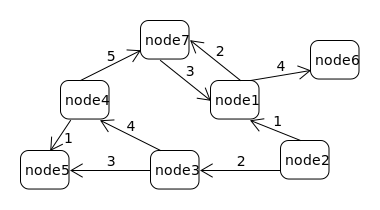
\includegraphics[width=\textwidth]{graphics/weightedDirectedNetwork.png}
        \subcaption{Weighted and directed graph.}
        \label{fig:simple_weighted_directed_network}
    \end{subfigure}\hfill
    \begin{subfigure}[b]{0.54\columnwidth}
        \centering
        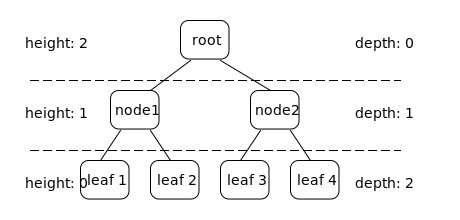
\includegraphics[width=\textwidth]{graphics/basicTree.png}
        \subcaption{Tree with a height of 2.}
        \label{fig:simple_tree}
    \end{subfigure}
    
    \caption{Schematic depictions of graph data structures.} % Remove the [...] argument if the original caption should be used in the figure list.
    \label{fig:intro} 
  \end{figure}

In conclusion, the most basic graph or network would be a simple unweighted and undirected set of nodes and links without any hierarchical relationship. To be able to represent different types of relationships in our data there exist different extensions of the core concept, such as trees and clustered graphs. 

\subsection{Graph Drawing}

As graph drawing is a subarea of information visualization, common knowledge from this research area can be applied here as well, with Shneiderman's visual information seeking mantra \label{seeking mantra} “Overview first, zoom and filter, then details-on-demand” \cite{shneiderman_eyes_1996} being one of the most famous. Additionally, the Gestalt Principles can also be used in graph drawing as Kobourov et al.
\cite{kobourov_gestalt_2015} shows. Gestalt Principles can be used to produce more aesthetically pleasing visualizations by defining drawing conventions and even improve the impression of the data. Cluster affiliation of nodes can be expressed by similar colors, shapes or simply by proximity, while the form of links should be consistent without any sharp bends.

For representation of data structures, node-link and space-filling concepts are the most important ones used in this thesis. Space-filling visualizations usually use multiscale approaches to encode hierarchical information (see Figure \ref{fig:hierarchicalCirclePlot}). Node-link diagrams tend to utilize force-based or constraint-based layouts\cite{von_landesberger_visual_2011}. Layout techniques are necessary to calculate the node positions. 
Force based\label{exp:force_based_background} layout techniques work without any domain-specific knowledge, therefore provide a flexible way to determine layouts for node-link graphs \cite{kobourov_spring_2012}. Only structural information about the graph relationships themselves are used. 
There are a variety of different approaches, but the general concept is always the same. 
These systems work by providing numerous repelling and attracting forces between nodes and links that update the position of the nodes. Usually these forces are related to Hooke's law. For example, an approach by Fruchterman et al. \cite{fruchterman_graph_1991} uses repulsive forces between all nodes and attraction forces for linked nodes.
The defined forces are then processed with a given set of nodes and links for either a limited number of iterations, a fixed time, some sort of dynamic condition (for instance the momentum of the nodes fall below a certain threshold) or just infinitely.
Large graphs, however, are a common problem as physical force models tend to have many local minima and therefore do not produce optimal results \cite{kobourov_spring_2012}.
Instead of defining interactions between nodes and links, constraints try to model the resulting layout directly; for instance, by placing nodes of certain groups in predefined locations of the screen.

Another form of graphs are multilayer visualizations\label{exp:multilayer}. Their goal is to combine multiple node-link diagrams, so-called layers into one visualization, including the relations between them. 
%A subset of proposed multilayer visualizations define the layers as an aspect of the dataset. The same node can be part of multiple aspects, multiple networks respectively.
Source and target layer of the links are well-defined, they can either be considered as intra-layer when the source and target layer are the same or inter-layer when they are not \cite{ghoniem_state_2019}. 
Since the nodes on multiple layers can represent the same entity, there are no strictly defined parent or child nodes in multilayer networks, therefore inter-layer links can be modeled between all layers.
%Another subset of proposed multilayer visualizations does not treat the individual layers as different aspects of the data. Instead, layers are used to combine multiple networks with different nodes in a single graph. This often makes their visualization concepts flexible to use.
When dealing with multiple graphs, there is a group structure that models the relations between nodes of different graphs.
Vehlow et al. \cite{vehlow_state_2015} differentiate group structures, in flat and hierarchical, as well as disjoint and overlapping aspects.
In overlapping datasets one node can be in multiple graphs at the same time. For example, a single person can be in a network of family-friends (layer/graph 1) and in a network of social-media friends (layer/graph 2).
In disjoint datasets, nodes are only part of one graph. These makes the visualizations more flexible to use.
\pagebreak

In our work we are dealing with a hierarchical and disjoint dataset. The hierarchical information can come from various clustering methods or be data inherent.

\section{VR Technology}
\label{chap:bg-vrtech}
Virtual Reality is by far not a new idea. In 1965, Sutherland \cite{Sutherland65theultimate} proposed an article of possibilities of future displays, including the “ultimate display” which allows a user to fully immerse in a virtual reality. Later, in 1992 we saw this concept as an early adoption by Cruz-Neira et al. \cite{cruz-neira_cave_1992} in the form of “The Cave”. It was a system with a head-mounted display which even allowed viewpoint tracking. The name giving “cave” was a setup of multiple screens driven by projectors placed on the walls, ceiling and floor around the user. The additional displays allowed multiple users at once to experience the virtual reality experience.  

Today, VR systems usually consist of a head mounted display (also called VR headset) and a pair of controllers, one for each hand. 
Degree of Freedom (DoF) describes how many geometric aspects are captured and can be used. Headsets with a DoF of three, like the Google Cardboard or Oculus Go, only allow tracking of rotational movement, e.g., looking around. 6-DOF Headsets, like the HTC Vive and Oculus Quest, also allow tracking translational movement and therefore enable the user to walk around in a virtual scene. 
While rotational tracking can be accomplishment by using gyroscopes inside the headset, translational tracking works either inside-out or outside-in. On inside-out concepts, the cameras and/or sensors are located on the headset itself as seen on the HTC Vive and Oculus Quest. Outside-in techniques instead place the cameras and/or sensors on stationary points in the room. Some examples are the original Oculus Rift and Playstation VR.
Some headsets use infrared emitters and sensors to determine the position while others rely on multiple camera feeds.
Giving all these different tracking capabilities of headsets, from a software frameworks point of view, VR systems are usually split into room-scale \label{exp:vr-experience}experiences where all tracking features are available, seating or standing experiences with no translational tracking and experiences with no user interaction and only rotational tracking for example a 360-degree video. In this work, we are interested in 6-DOF Headsets that support room-scale as well as seated and standing experiences.